\documentclass[10pt]{beamer}

\mode<presentation>{% Settings
    % link to view http://www.hartwork.org/beamer-theme-matrix/
    % ------------------------------------------------------------------------------
    % Slide Themes
    % ------------------------------------------------------------------------------
    %\usetheme{default}
    %\usetheme{AnnArbor}
    %\usetheme{Antibes}
    %\usetheme{Bergen}
    \usetheme{Berkeley}
    %\usetheme{Berlin}
    %\usetheme{Boadilla}
    %\usetheme{CambridgeUS}
    %\usetheme{Copenhagen}
    %\usetheme{Darmstadt}
    %\usetheme{Dresden}
    %\usetheme{Frankfurt}
    %\usetheme{Goettingen}
    %\usetheme{Hannover}
    %\usetheme{Ilmenau}
    %\usetheme{JuanLesPins} % rounded title, gradient at top with section, no bottom bar
    %\usetheme{Luebeck}     % square title, toc at top of each slide
    %\usetheme{Madrid}      % rounded title
    %\usetheme{Malmoe}
    %\usetheme{Marburg}
    %\usetheme{Montpellier}
    %\usetheme{PaloAlto}
    %\usetheme{Pittsburgh}
    %\usetheme{Rochester}
    %\usetheme{Singapore}
    %\usetheme{Szeged}
    %\usetheme{Warsaw}

    % ------------------------------------------------------------------------------
    % Color Schemes
    % ------------------------------------------------------------------------------
    %\usecolortheme{default}
    %\usecolortheme{albatross}  % blue background with darker blue
    %\usecolortheme{beaver}     % gray with red
    %\usecolortheme{beetle}     % gray background
    %\usecolortheme{crane}      % orange
    \usecolortheme{dolphin}     % white with purple
    %\usecolortheme{dove}       % all white
    %\usecolortheme{fly}        % all gray including background
    %\usecolortheme{lily}       % white with blue
    %\usecolortheme{orchid}     % default blue
    %\usecolortheme{rose}       % default blue
    %\usecolortheme{seagull}    % darker gray than seahorse
    %\usecolortheme{seahorse}   % light gray blueish tint
    %\usecolortheme{whale}      % default blue
    %\usecolortheme{wolverine}  % yellow with a little blue

    %\setbeamertemplate{footline} % To remove the footer line in all slides uncomment this line
    %\setbeamertemplate{footline}[page number] % To replace the footer line in all slides with a simple slide count uncomment this line
    \setbeamertemplate{navigation symbols}{} % To remove the navigation symbols from the bottom of all slides uncomment this line
    \setbeamertemplate{bibliography item}{\insertbiblabel} % to number bibliography entries
}

\usepackage{Logemann}
\usepackage{Integral}
\usepackage{LinearAlgebra}
\usepackage{Derivative}
\usepackage{Vector}
\usepackage{Sum}
\usepackage{SetTheory}
\usepackage{booktabs}
\usepackage{amsmath}
\usepackage[backend=biber]{biblatex}
\addbibresource{refs.bib}

\title[]{Local Discontinuous Galerkin Method for Solving Thin Film Equations} % The short title
% appears at the bottom of every slide, the full title is only on the title page

\author{Caleb Logemann \and James Rossmanith} % Your name
\institute[Iowa State University]{% Your institution as it will appear on the bottom of every slide, may be shorthand to save space
Mathematics Department,\\ Iowa State University \\ % Your institution for the title page 
\medskip
\textit{logemann@iastate.edu}} % Your email address

\date{\today} % Date, can be changed to a custom date


\begin{document}
  \begin{frame}
    \titlepage{}
  \end{frame}

  \begin{frame}
    \frametitle{Overview}
    \tableofcontents
  \end{frame}

  \section{Introduction}
    \begin{frame}
      \frametitle{Motivation}
      \begin{itemize}
        \item Aircraft Icing
        \item Runback
      \end{itemize}
      \begin{center}
        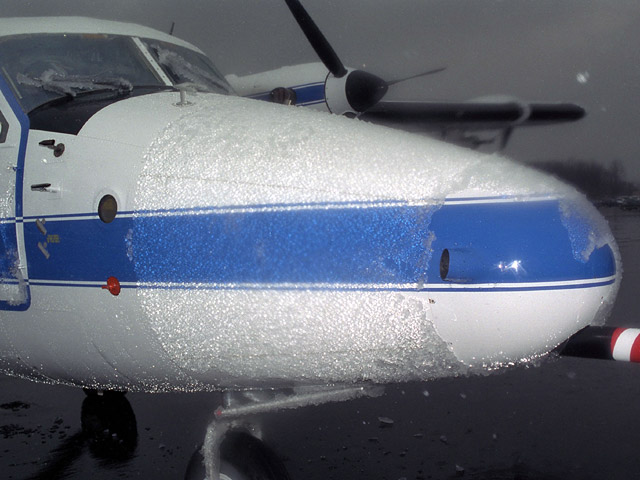
\includegraphics[scale=0.2]{Figures/Icing_on_a_plane.jpg}
        \hspace{0.1in}
        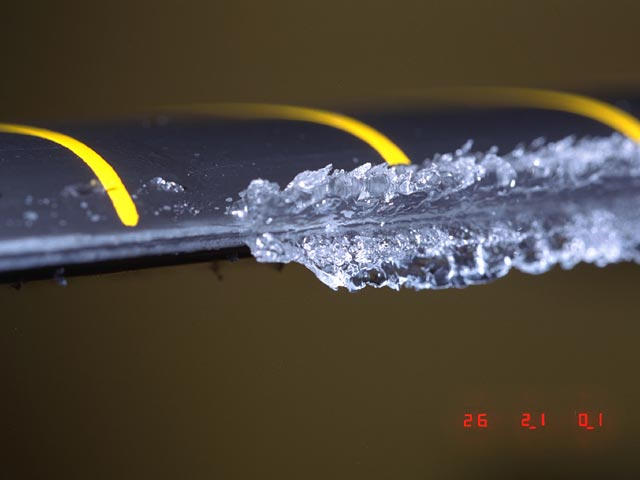
\includegraphics[scale=0.2]{Figures/Icing_on_a_rotor.jpg}
      \end{center}
      \begin{itemize}
        \item Industrial Coating
      \end{itemize}
    \end{frame}

  \section{Derivation}
    \begin{frame}
      \frametitle{Model Equations}
      \begin{itemize}
        \item Navier-Stokes Equation
          \begin{align*}
            \nabla \cdot \v{u} &= 0 \\
            \partial_t \v{u} + \nabla \cdot \p{\v{u}\v{u}} &= - \frac{1}{\rho} \nabla p + \frac{1}{\rho}\nabla \cdot \sigma + \v{g} \\
            \partial_t h_s + \p{u, v}^T \cdot \nabla h_s &= w \\
            \partial_t h_b + \p{u, v}^T \cdot \nabla h_b &= w
          \end{align*}
        \item Lubrication or reduced Reynolds number approximation
        \item Thin-Film Equation - 1D with $q$ as fluid height.
          \[
            q_t + \p{f(x, t) q^2 - g(x, t) q^3}_x = -\p{h(x, t) q^3 q_{xxx}}_x
          \]
      \end{itemize}
    \end{frame}

  \section{Method}
    \begin{frame}
      \begin{itemize}
        \frametitle{Method Overview}
        \item Simplified Model
          \[
            q_t + \p{q^2 - q^3}_x = -\p{q^3 q_{xxx}}_x \qquad \p{0, T} \times \Omega
          \]

        \item Runge Kutta Implicit Explicit (IMEX)
          \begin{align*}
            q_t &= F(q) + G(q)
          \end{align*}
          \begin{itemize}
            \item F evaluated explicitly
            \item G solved implicitly
          \end{itemize}
          \begin{align*}
            F(q) &= -\p{q^2 - q^3}_x  \\
            G(q) &= \p{q^3 q_{xxx}}_x 
          \end{align*}

      \end{itemize}
    \end{frame}

  \subsection{Convection}
    \begin{frame}
      \frametitle{Convection}
      \begin{itemize}
        \item Convection Equation
          \begin{gather*}
            F(q) = f\p{q}_x = 0 \qquad \p{0, T} \times \Omega \\
            f(q) = q^2 - q^3
          \end{gather*}

        \item Weak Form \hfill \\
          Find $q$ such that
          \[
            \dintt*{\Omega}{}{F(q) v - f(q) v_x}{x} + \eval{\hat{f}v}{\partial\Omega} = 0
          \]
          for all test functions $v$
      \end{itemize}
    \end{frame}

    \begin{frame}
      \frametitle{Notation}
      \begin{itemize}
        \item Partition the domain, $\br{a, b}$ as
          \[
            a = x_{1/2} < \cdots < x_{j-1/2} < x_{j+1/2} < \cdots < x_{N + 1/2} = b
          \]

        \item $I_j = \br{x_{j-1/2}, x_{j+1/2}}$
        \item $x_j = \frac{x_{j+1/2} + x_{j-1/2}}{2}$.
          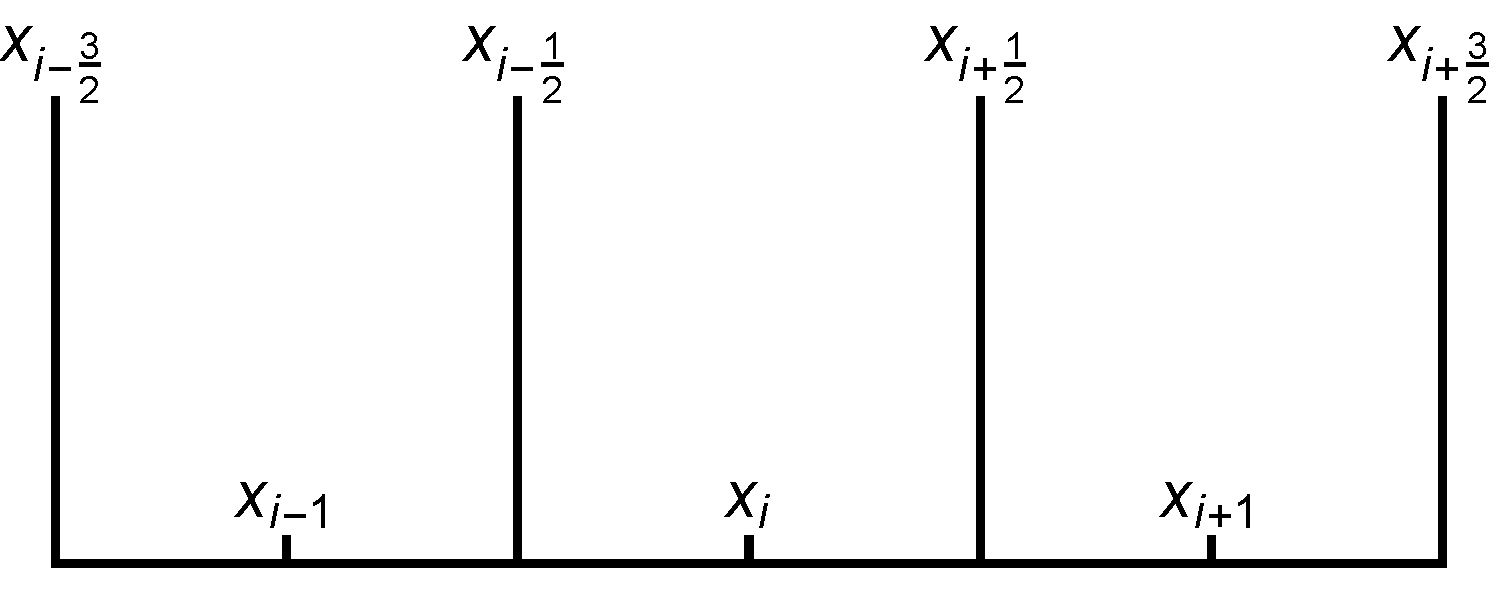
\includegraphics[scale=0.35]{Figures/Cells.pdf}
      \end{itemize}
    \end{frame}

    \begin{frame}
      \frametitle{Runge Kutta Discontinuous Galerkin}
      \begin{itemize}
        \item 
          Find $Q(t,x)$ such that for each time $t \in \p{0, T}$, $Q(t, \cdot) \in V_h = \set{v \in L^1(\Omega): \eval{v}{I_j} \in P^k(I_j)}$
          \begin{align*}
            \dintt{I_j}{}{F(Q) v}{x} &= \dintt{I_j}{}{f(Q)v_x}{x} \\
            &- \p{\mcF_{j + 1/2}v^-(x_{j+1/2}) - \mcF_{j - 1/2}v^+(x_{j-1/2})}
          \end{align*}
          for all $v \in V_h$

        \item Rusanov/Local Lax-Friedrichs Numerical Flux
          \small{\[
            \mcF_{j+1/2} = \frac{1}{2}\p{f\p{Q^-_{j+1/2}} + f\p{Q^+_{j+1/2}}} + \frac{1}{2}\max[q]{\abs{f'(q)}}\p{Q^-_{j+1/2} - Q^+_{j+1/2}}
          \]}
      \end{itemize}
    \end{frame}

  \subsection{Diffusion}
    \begin{frame}
      \frametitle{Diffusion}
      \begin{itemize}
        \item Diffusion Equation
          \begin{align*}
            G(q) &= -\p{q^3 q_{xxx}}_x \qquad \p{0, T} \times \Omega
          \end{align*}

        \item Local Discontinuous Galerkin
          \begin{align*}
            r &= q_x \\
            s &= r_x \\
            u &= s_x \\
            G(q) &= \p{q^3 u}_x
          \end{align*}
      \end{itemize}
    \end{frame}

    \begin{frame}
      \frametitle{Local Discontinuous Galerkin}
      Find $Q(t, x), R(x), S(x), U(x)$ such that for all $t \in \p{0, T}$
      $Q(t, \cdot), R, S, U \in V_h = \set{v \in L^1(\Omega): \eval{v}{I_j} \in P^k(I_j)}$
      \begin{align*}
        \dintt{I_j}{}{R v}{x} &= -\dintt{I_j}{}{Q v_x}{x} + \p{\hat{Q}_{j+1/2}v^-_{j+1/2} - \hat{Q}_{j-1/2} v^+_{j-1/2}} \\
        \dintt{I_j}{}{S w}{x} &= -\dintt{I_j}{}{R w_x}{x} + \p{\hat{R}_{j+1/2}w^-_{j+1/2} - \hat{R}_{j-1/2} w^+_{j-1/2}} \\
        \dintt{I_j}{}{U y}{x} &= -\dintt{I_j}{}{S y_x}{x} + \p{\hat{S}_{j+1/2}y^-_{j+1/2} - \hat{S}_{j-1/2} y^+_{j-1/2}} \\
        \dintt{I_j}{}{G(Q) z}{x} &= -\dintt{I_j}{}{Q^3 U z_x}{x} + \p{\hat{U}_{j+1/2}z^-_{j+1/2} - \hat{U}_{j-1/2} z^+_{j-1/2}}
      \end{align*}
      for all $I_j \in \Omega$ and all $v, w, y, z \in V_h$.
    \end{frame}

    \begin{frame}
      \frametitle{Numerical Fluxes}
      \begin{align*}
        \hat{Q}_{j+1/2} &= Q^+_{j+1/2} \\
        \hat{R}_{j+1/2} &= R^-_{j+1/2} \\
        \hat{S}_{j+1/2} &= S^+_{j+1/2} \\
        \hat{U}_{j+1/2} &= \p{Q^3 U}^-_{j+1/2}
      \end{align*}
      \begin{center}
        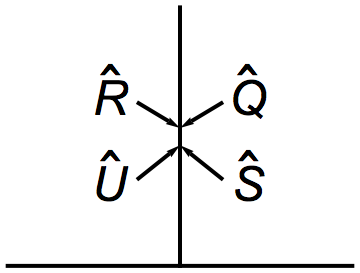
\includegraphics[scale=0.3]{Figures/localDG.png}
      \end{center}
    \end{frame}

    \begin{frame}
      \frametitle{IMEX Runge Kutta}
      \begin{itemize}
        \item IMEX scheme
          \begin{align*}
            q^{n+1} &= q^n + \Delta t \sum{i = 1}{s}{b_i' F(t_i, u_i)} + \Delta t \sum{i=1}{s}{b_i G(t_i, u_i)} \\
            u_i &= q^n + \Delta t \sum{j = 1}{i-1}{a_{ij}' F(t_j, u_j)} + \Delta t \sum{j=1}{i}{a_{ij} G(t_j, u_j)} \\
            t_i &= t^n + c_i \Delta t
          \end{align*}

        \item Double Butcher Tableaus \hfill \\ \hfill \\
          \begin{tabular}{r|l}
            $c'$ & $a'$ \\
            \midrule
               & $b'^T$
          \end{tabular}
          \begin{tabular}{r|l}
            $c$ & $a$ \\
            \midrule
               & $b^T$
          \end{tabular}
      \end{itemize}
    \end{frame}

    \begin{frame}
      \begin{itemize}
        \item 1st Order - L-Stable SSP \hfill \\ \hfill \\
          \begin{tabular}{r|l}
            0 & 0 \\
            \midrule
              & 1 
          \end{tabular}\hspace{0.5cm}
          \begin{tabular}{r|l}
            1 & 1 \\
            \midrule
              & 1 
          \end{tabular}

        \vspace{0.5cm}

        \item 2nd Order - SSP \hfill \\ \hfill \\
          \begin{tabular}{r|lll}
            0 & 0 & 0 & 0 \\
            0 & 0 & 0 & 0 \\
            1 & 0 & 1 & 0 \\
            \midrule
              & 0 & $\frac{1}{2}$ & $\frac{1}{2}$ \\
          \end{tabular}\hspace{0.5cm}
          \begin{tabular}{r|lll}
            $\frac{1}{2}$ & $\frac{1}{2}$ & 0 & 0 \\
            0 & $-\frac{1}{2}$ & $\frac{1}{2}$ & 0 \\
            1 & 0 & $\frac{1}{2}$ & $\frac{1}{2}$ \\
            \midrule
              & 0 & $\frac{1}{2}$ & $\frac{1}{2}$ \\
          \end{tabular}
      \end{itemize}
    \end{frame}

    \begin{frame}
      \begin{itemize}
        \item 3rd Order - L-Stable SSP \hfill \\ \hfill \\
          \begin{tabular}{r|llll}
            0 & 0 & 0 & 0 & 0 \\
            0 & 0 & 0 & 0 & 0 \\
            1 & 0 & 1 & 0 & 0 \\
            $\frac{1}{2}$ & 0 & $\frac{1}{4}$ & $\frac{1}{4}$ & 0 \\
            \midrule
              & 0 & $\frac{1}{6}$ & $\frac{1}{6}$ & $\frac{2}{3}$ \\
          \end{tabular} \hspace{0.5cm}
          \begin{tabular}{r|llll}
            $\alpha$ & $\alpha$ & 0 & 0 & 0 \\
            0 & -$\alpha$ & $\alpha$ & 0 & 0 \\
            1 & 0 & $1 - \alpha$ & $\alpha$ & 0 \\
            $\frac{1}{2}$ & $\beta$ & $\eta$ & $\zeta$ & $\alpha$ \\
            \midrule
              & 0 & $\frac{1}{6}$ & $\frac{1}{6}$ & $\frac{2}{3}$ \\
          \end{tabular} \\
          \begin{align*}
            \alpha &= 0.24169426078821 \\
            \beta &= 0.06042356519705 \\
            \eta &= 0.1291528696059 \\
            \zeta &= \frac{1}{2} - \beta - \eta - \alpha
          \end{align*}
      \end{itemize}
    \end{frame}

    \begin{frame}
      \frametitle{Nonlinear Solvers}
      \begin{itemize}
        \item Nonlinear System
          \begin{align*}
            u_i - a_{ii} \Delta t G(u_i) &= b
          \end{align*}

        \item Picard Iteration
          \begin{align*}
            \tilde{G}(q, u) &= (q^3 u_{xxx})_x 
          \end{align*}
          \begin{gather*}
            u_0 = q^n  \qquad u_i^0 = u_{i-1} \\
            u_i^j - a_{ii} \Delta t \tilde{G}(u_i^{j-1}, u_i^j) = b
          \end{gather*}

        \item Number of picard iterations equals order in time and space
      \end{itemize}
    \end{frame}

  \section{Numerical Results}
    \begin{frame}
      \frametitle{Manufactured Solution}
      \begin{align*}
        q_t + (q^2 - q^3)_x &= -\p{q^3 q_{xxx}}_x + s(x,t) \\
        q(x, t) &= 0.1*\sin{2\pi(x - t)} + 0.15
      \end{align*}
      \begin{center}
      \begin{tabular}{rll}
        \toprule
        \multicolumn{3}{c}{1st Order IMEX} \\
        \midrule
        $N$ &  error &  order \\
        \midrule
         50  & 0.0278  & -  \\
         100 & 0.0144  & 0.955   \\
         200 & 0.0072  & 0.988 \\
        \bottomrule
      \end{tabular}
      \end{center}
    \end{frame}

    \begin{frame}
      \frametitle{Manufactured Solution}
      \begin{align*}
        q_t + (q^2 - q^3)_x &= -\p{q^3 q_{xxx}}_x + s(x,t) \\
        q(x, t) &= 0.1*\sin{2\pi(x - t)} + 0.15
      \end{align*}
      \begin{center}
      \begin{tabular}{rll}
        \toprule
        \multicolumn{3}{c}{2nd Order IMEX} \\
        \midrule
        $N$ &  error &  order \\
        \midrule
         20 & 0.00265  & -  \\
         40 & 0.000689  & 1.94 \\
         80 & 0.000184  & 1.91 \\
        \bottomrule
      \end{tabular}
      \end{center}
    \end{frame}

    \begin{frame}
      \frametitle{Manufactured Solution}
      \begin{align*}
        q_t + (q^2 - q^3)_x &= -\p{q^3 q_{xxx}}_x + s(x,t) \\
        q(x, t) &= 0.1*\sin{2\pi(x - t)} + 0.15
      \end{align*}
      \begin{center}
      \begin{tabular}{rll}
        \toprule
        \multicolumn{3}{c}{3rd Order IMEX} \\
        \midrule
        $N$ &  error &  order \\
        \midrule
         20 & 6.57 $\times 10^{-5}$ & -  \\
         40 & 8.35 $\times 10^{-6}$ & 2.97 \\
         80 & 1.07 $\times 10^{-6}$ & 2.96 \\
        \bottomrule
      \end{tabular}
      \end{center}
    \end{frame}

    \begin{frame}
      \frametitle{Observations}
      \begin{itemize}
        \item CFL Restrictions
        \item 1st Order - 0.15
        \item 2nd Order - 0.05
        \item 3rd Order - 0.01

        \item Linearized Problem
          \begin{align*}
            q_t + (q^2 - q^3)_x &= -(f(x, t) q_xxx)_x + s(x, t) \\
            f(x, t) &= \p{\tilde{q}(x, t)}^3
          \end{align*}

        \item Same CFL restrictions
      \end{itemize}
    \end{frame}

    \begin{frame}
      \frametitle{Wave Structure with Nonlinear Hyper Diffusion}
      \[
        q_t + \p{q^2 - q^3}_x = -\p{q^3q_{xxx}}_x
      \]
      \[
        q_r = 0.1 \qquad q_l = 0.3
      \]
      \begin{center}
        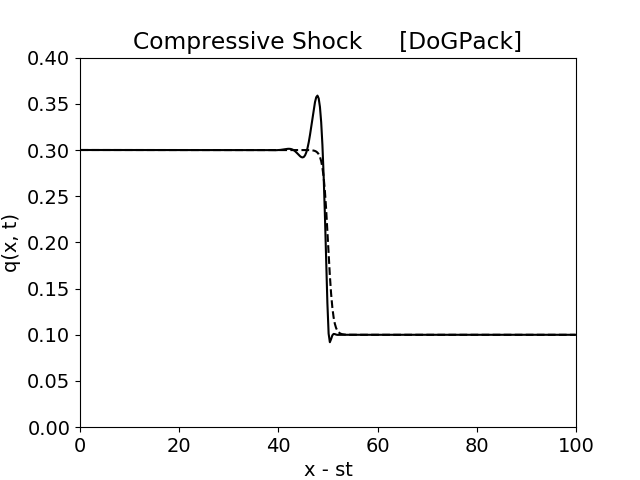
\includegraphics[scale=0.4]{Figures/case1.png}
      \end{center}
    \end{frame}

    \begin{frame}
      \frametitle{Wave Structure with Nonlinear Hyper Diffusion}
      \[
        q_r = 0.1 \qquad q_l = 0.3323
      \]
      \[
        q(x, 0) = \p{-\tanh{x - 50} + 1}\frac{q_l - q_r}{2} + q_r
      \]
      \begin{center}
        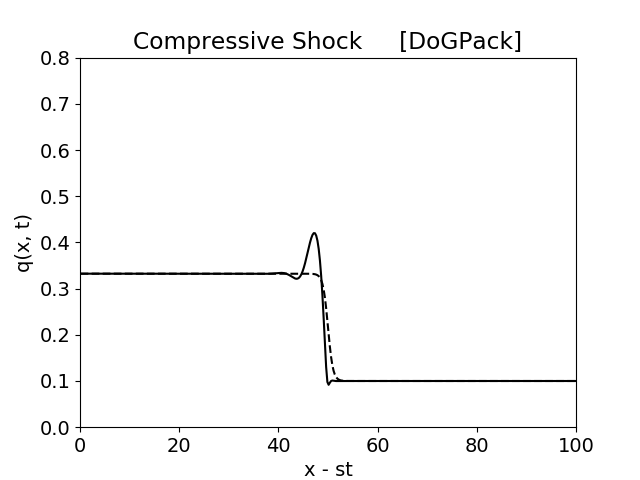
\includegraphics[scale=0.4]{Figures/case2_1.png}
      \end{center}
    \end{frame}

    \begin{frame}
      \frametitle{Wave Structure with Nonlinear Hyper Diffusion}
      \[
        q_r = 0.1 \qquad q_l = 0.3323 \qquad q_m = 0.6
      \]
      \[
        q(x, 0) = 
        \begin{cases}
          \frac{q_m - q_l}{2}\tanh{x - 50} + \frac{q_m + q_l}{2} & x < 55 \\
          -\frac{q_m - q_r}{2}\tanh{x - 60} + \frac{q_m + q_r}{2} + q_r & x > 55 \\
        \end{cases}
      \]
      \begin{center}
        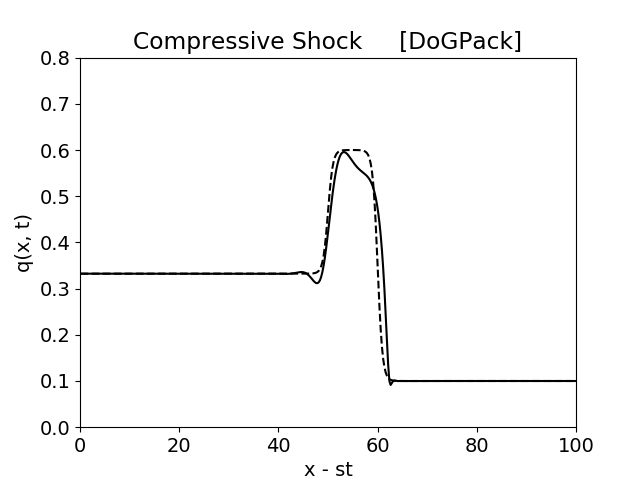
\includegraphics[scale=0.4]{Figures/case2_2.png}
      \end{center}
    \end{frame}

    \begin{frame}
      \frametitle{Wave Structure with Nonlinear Hyper Diffusion}
      \[
        q_r = 0.1 \qquad q_l = 0.4
      \]
      \[
        q(x, 0) = \p{-\tanh{x - 300} + 1}\frac{q_l - q_r}{2} + q_r
      \]
      \begin{center}
        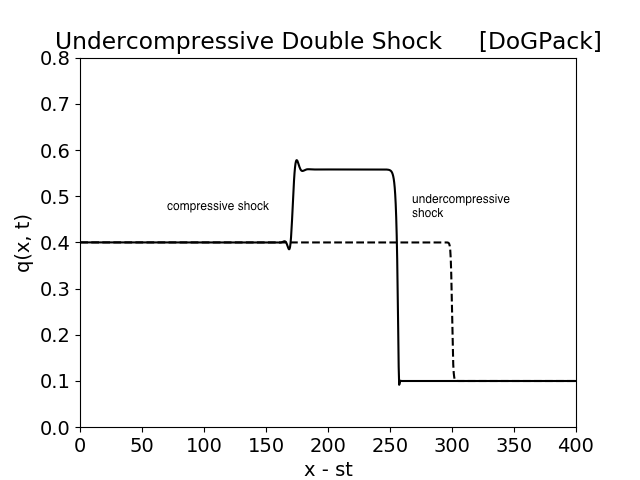
\includegraphics[scale=0.4]{Figures/case3.png}
      \end{center}
    \end{frame}

    \begin{frame}
      \frametitle{Wave Structure with Nonlinear Hyper Diffusion}
      \[
        q_r = 0.1 \qquad q_l = 0.8
      \]
      \[
        q(x, 0) = \p{-\tanh{x - 1100} + 1}\frac{q_l - q_r}{2} + q_r
      \]
      \begin{center}
        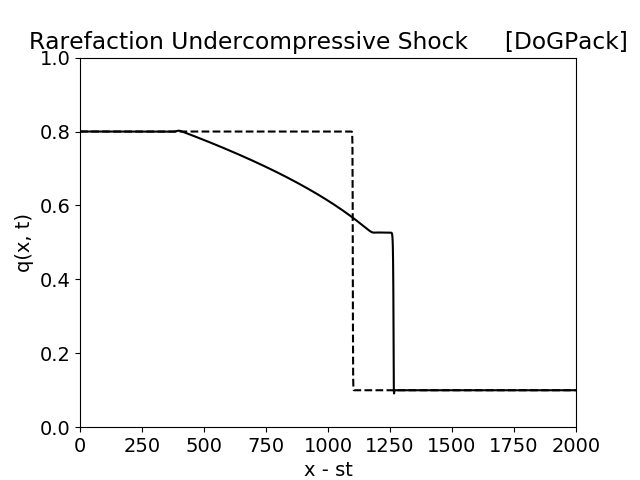
\includegraphics[scale=0.4]{Figures/case4.png}
      \end{center}
    \end{frame}

  \section{Conclusion}
    \begin{frame}
      \frametitle{Conclusion}
      Observations
      \begin{itemize}
        \item Expensive computations
        \item Nonlinear Hyper Diffusion has subtle instabilities
      \end{itemize}
      Future Work
      \begin{itemize}
        \item Hybridized Discontinuous Galerkin Method
      \end{itemize}
    \end{frame}

    \begin{frame}[allowframebreaks]
      \frametitle{Bibliography}
      \nocite{*}
      \printbibliography{}
    \end{frame}
\end{document}
